% This is samplepaper.tex, a sample chapter demonstrating the
% LLNCS macro package for Springer Computer Science proceedings;
% Version 2.21 of 2022/01/12
%
\documentclass[runningheads]{llncs}
%
\usepackage[T1]{fontenc}
% T1 fonts will be used to generate the final print and online PDFs,
% so please use T1 fonts in your manuscript whenever possible.
% Other font encondings may result in incorrect characters.
%
\usepackage{graphicx}
\usepackage{amssymb, amsmath}
\usepackage{tikz}
\usetikzlibrary{arrows.meta, positioning, calc}
% Used for displaying a sample figure. If possible, figure files should
% be included in EPS format.
%
% If you use the hyperref package, please uncomment the following two lines
% to display URLs in blue roman font according to Springer's eBook style:
%\usepackage{color}
%\renewcommand\UrlFont{\color{blue}\rmfamily}
%\urlstyle{rm}
%
\begin{document}
%
\title{Dynamic Financial Ontology: Bridging Heterogeneous Market Events 
and Co-movement Structure with Temporal Graph Networks}
%
\titlerunning{DyFO: Stateless Temporal Graph Attention for Financial Co-movement}
% If the paper title is too long for the running head, you can set
% an abbreviated paper title here
%
\author{First Author\inst{1}\orcidID{0000-1111-2222-3333} \and
Second Author\inst{2,3}\orcidID{1111-2222-3333-4444} \and
Third Author\inst{3}\orcidID{2222--3333-4444-5555}}
%
\authorrunning{F. Author et al.}
% First names are abbreviated in the running head.
% If there are more than two authors, 'et al.' is used.
%
\institute{Princeton University, Princeton NJ 08544, USA \and
Springer Heidelberg, Tiergartenstr. 17, 69121 Heidelberg, Germany
\email{lncs@springer.com}\\
\url{http://www.springer.com/gp/computer-science/lncs} \and
ABC Institute, Rupert-Karls-University Heidelberg, Heidelberg, Germany\\
\email{\{abc,lncs\}@uni-heidelberg.de}}
%
\maketitle              % typeset the header of the contribution
%
\begin{abstract}
Forecasting dynamic financial co-movements requires integrating asynchronous signals into a continuous-time relational model. We propose \textbf{DyFO} (Dynamic Financial Observer), a stateless Temporal Graph Attention Network (TGAT)~\cite{xu2020inductive} over a heterogeneous graph with three edge types: DCC-GARCH dynamic correlations (\texttt{CORR}), sector links (\texttt{SECT}), and Fama--French five-factor co-loadings (\texttt{FACT}). Evaluated on 50 S\&P~500 constituents spanning all 11 GICS sectors (2018--2024) under a rigorous nine-window walk-forward protocol (1{,}093 out-of-sample days), DyFO achieves strong and consistent predictive accuracy (\(R^2=0.891\), Spearman \(\rho=0.959\), MAE \(=0.036\), F1 \(=0.793\)), outperforming a recurrent Temporal Graph Network (TGN), a ROLAND-style temporal snapshot baseline, and a static GAT across all windows. Diebold--Mariano tests with Newey--West HAC correction yield \(p < 10^{-121}\) for all comparisons involving temporal models, with effect sizes \(|d| > 2.2\); all results remain significant after Holm--Bonferroni correction. In downstream portfolio evaluation under a Global Minimum Variance strategy with paired block bootstrap (2{,}000 iterations), Sharpe differences are not statistically distinguishable---consistent with the well-documented error-amplification pathology of mean-variance optimisation. Overall, the results show that stateless temporal graph attention provides clear and reproducible gains in correlation forecasting over recurrent and snapshot-based alternatives, while highlighting the need for decision-aware allocation strategies to translate predictive improvements into portfolio utility.
\end{abstract}
%
%
%

\section{Introduction}\label{sec:introduction}


Portfolio management consists in periodically reallocating capital across a set of assets so as to maximise long-term returns while controlling risk. Accurate modelling of asset co-movements is central to this task, since the covariance (or correlation) matrix directly determines the risk of any portfolio. Traditional approaches rely on rolling-window Pearson correlations or parametric models such as the Dynamic Conditional Correlation GARCH (DCC-GARCH) of \cite{engle2002dynamic}. Although effective at capturing volatility clustering, these methods treat each pair of assets in isolation and therefore cannot exploit the rich relational structure that exists among companies---sector membership, supply-chain links, or shared exposure to macroeconomic factors.

Recent years have witnessed a surge of interest in graph-based and reinforcement-learning methods for portfolio management. Several works have modelled inter-company relationships as static graphs and employed graph neural networks to improve feature representations. Notable examples include the Relational Graph Convolutional Network (R-GCN) framework of \cite{shi2022gpm} (GPM), which combines multi-scale temporal convolutions with relational propagation over sector-industry and Wikidata links, and the Cross-Asset Attention Network of \cite{wang2019alphastock} (AlphaStock). While these approaches demonstrate the value of relational information, they typically operate on \emph{static} graphs and output portfolio weights directly through an end-to-end reinforcement-learning policy. Consequently, they lack an explicit, causally valid forecast of the full correlation matrix and cannot be rigorously evaluated through statistical tests on out-of-sample covariance prediction.

In this paper we introduce \textbf{DyFO} (Dynamic Financial Observer), a Temporal Graph Network that bridges heterogeneous market events and co-movement structure for next-day pairwise correlation forecasting. DyFO operates on a \emph{dynamic} heterogeneous graph whose edges evolve daily: DCC-GARCH correlations (\texttt{CORR}), GICS sector links (\texttt{SECT}), and Fama--French five-factor co-loadings (\texttt{FACT}). Market activity is modelled as a continuous stream of typed events (price updates, earnings releases, macro surprises, Federal Reserve decisions, etc.), each carrying a three-dimensional feature vector. A stateless Temporal Graph Attention Network (TGAT)~\cite{xu2020inductive} encodes recent events into node states,
sidestepping the ``cold start'' instabilities of recurrent mechanisms,
while a single-layer multi-head graph attention layer aggregates information over the static relational neighbourhood. The resulting node embeddings feed a lightweight decoder that predicts the full 30×30 correlation matrix for the next trading day.

We evaluate DyFO on 50 S\&P~500 large-cap constituents spanning all 11 GICS sectors over the period 2018--2024, employing a rigorous nine-window non-overlapping walk-forward protocol that yields 1{,}093 out-of-sample trading days. DyFO achieves \(R^2 = 0.891\), Spearman \(\rho = 0.959\), MAE \(= 0.036\), and classification F1 \(= 0.793\) for high-correlation pairs, consistently outperforming a recurrent TGN baseline~\cite{rossi2020temporal}, a ROLAND-style snapshot baseline~\cite{you2022roland}, and a static GAT across all nine windows. Diebold--Mariano tests with Newey--West HAC correction confirm significant predictive superiority (DM \(= -23.5\), \(p < 10^{-121}\) vs.\ TGN; DM \(= -55.5\), \(p \approx 0\) vs.\ ROLAND), with all results surviving Holm--Bonferroni correction. Block-bootstrap portfolio evaluation (Global Minimum Variance allocation, 2{,}000 iterations, 5-day blocks) yields non-significant Sharpe differences across all model pairs---indicating that improved covariance forecasting should be paired with allocation strategies explicitly aligned with forecast quality.

The main contributions of this work are threefold:
\begin{itemize}
    \item We propose the first domain-adapted Temporal Graph Attention Network (TGAT)~\cite{xu2020inductive} for continuous-time financial event streams, extending the original homogeneous formulation with three key innovations: (i)~typed edge embeddings that distinguish correlation, sector, and factor relations; (ii)~a heterogeneous event vocabulary with domain-specific feature vectors; and (iii)~a continuous regression decoder for pairwise correlation forecasting. The resulting stateless architecture resolves recurrent memory instabilities and enables highly accurate next-day predictions on a dynamic heterogeneous graph.
    \item We integrate three complementary edge types---dynamic correlations, sector membership, and factor co-loadings---and demonstrate that each contributes measurably to predictive accuracy.
    \item We provide the first rigorous statistical evaluation of graph-based correlation models via Diebold--Mariano, Wilcoxon signed-rank, and block-bootstrap Sharpe-ratio tests with Newey--West HAC standard errors, establishing robust superiority over strong baselines.
\end{itemize}

The remainder of the paper is organised as follows. Section~\ref{sec:related} reviews related work on graph-based and temporal models for portfolio management. Section~\ref{sec:methodology} formalises the problem and details the DyFO architecture. Section~\ref{sec:experiments} presents the experimental setup and main results. Finally, Section~\ref{sec:conclusion} concludes and outlines future research directions.

\section{Related Work}\label{sec:related}

Portfolio management has traditionally been addressed through two complementary lines of research: classical optimisation techniques and, more recently, data-driven learning methods.

\paragraph{Classical approaches.}
Markowitz's mean-variance framework \cite{markowitz1952} remains the foundation of modern portfolio theory, selecting assets that minimise variance for a target return. Subsequent refinements introduced shrinkage estimators, robust optimisation, and factor models. The Fama--French five-factor model \cite{fama2015fivefactor} is now widely used to capture systematic risk exposures. For dynamic settings, Engle's DCC-GARCH model \cite{engle2002dynamic} provides time-varying conditional correlations that are still considered a strong baseline in the industry. These methods, however, treat pairwise relationships in isolation and cannot exploit higher-order relational structures among companies.

\paragraph{Deep reinforcement learning for portfolio management.}
The advent of deep RL opened the possibility of learning policies directly from market data. Early works such as the Ensemble of Identical Independent Evaluators (EIIE) \cite{jiang2017deepreinforcementlearningframework} and its multi-scale extension EI³ \cite{shi2019multiscale} employed convolutional networks to extract price features and output portfolio weights. Subsequent improvements include the Portfolio Policy Network (PPN) \cite{zhang2020cost}, which adds a temporal correlational convolution block, and State-Augmented RL (SARL) \cite{ye2020reinforcement}, which augments states with external signals such as financial news. While effective, these approaches rely solely on price histories and ignore explicit inter-company relationships.

\paragraph{Graph-based methods in finance.}
Recognising that companies are embedded in a rich relational structure, several authors have modelled markets as graphs. AlphaStock \cite{wang2019alphastock} introduced a Cross-Asset Attention Network to capture inter-stock dependencies. The Relational Stock Ranking (RSR) model \cite{feng2019temporal} proposed a temporal graph convolution that jointly models price evolution and static relations. Hierarchical Attention Networks for Stock prediction (HATS) \cite{kim2019hatshierarchicalgraphattention} and Multi-GCGRU \cite{ye2020multi} further enriched node representations with industry, shareholding, and topicality edges. More recently, DeepPocket \cite{soleymani2021deeppocket} applied a standard GCN over financial instruments, while the GPM framework of \cite{shi2022gpm} combined multi-scale temporal convolutions with an R-GCN over heterogeneous company relations (sector-industry and Wikidata links) and introduced temperature-scaled softmax for portfolio diversity.

All the aforementioned graph-based methods share two important limitations when applied to portfolio management. First, the underlying graphs are \emph{static}: edge weights or even edge existence do not evolve with market conditions. Second, most works output portfolio weights directly through an end-to-end policy, making it difficult to isolate the quality of the learned correlation structure or to apply classical risk-optimisation techniques downstream.

\paragraph{Temporal Graph Networks and TGAT.}
To capture the inherently dynamic nature of financial markets, Temporal Graph Networks (TGN) were introduced by \cite{rossi2020temporal}. TGN maintains a memory vector per node that is updated continuously as events arrive via a GRU cell, and propagates information over both temporal and structural neighbourhoods. The Temporal Graph Attention Network (TGAT)~\cite{xu2020inductive} offered a stateless alternative, replacing recurrent memory with a functional time encoding and multi-head self-attention over temporal neighbourhoods, thereby avoiding the cold-start instabilities inherent to GRU-based state propagation. A third line, ROLAND \cite{you2022roland}, operates on discrete graph snapshots and propagates hidden states between them via exponential moving averages. DySAT~\cite{sankar2020dysat} similarly employs discrete snapshots but replaces EMA propagation with self-attention across the snapshot sequence, operating on homogeneous graphs without typed edge semantics.

While these architectures have shown strong results on generic dynamic graph benchmarks, they share several limitations when applied to financial correlation forecasting. First, they were designed for \emph{homogeneous} graphs with a single edge type and do not natively support heterogeneous relational semantics. Second, their event representations lack domain-specific structure---financial event types (earnings, macro surprises, rate decisions) carry fundamentally different information, yet are treated uniformly in the original formulations. Third, they target link classification or node-level tasks, not continuous regression over a full pairwise correlation matrix.

A complementary line of work addresses financial prediction through probabilistic factor models. FactorVAE~\cite{duan2022factorvae} integrates a dynamic factor model with a variational autoencoder, learning latent factors from noisy cross-sectional return data via a prior-posterior training scheme. While effective for \emph{return prediction}, FactorVAE operates on homogeneous price-volume features without relational graph structure and does not target the pairwise correlation matrix that is central to covariance-based portfolio optimisation---a fundamentally different objective from the one pursued here.

DyFO builds upon and extends the TGAT paradigm to address these gaps. Specifically, it introduces (i)~typed edge embeddings that distinguish correlation (\texttt{CORR}), sector (\texttt{SECT}), and factor (\texttt{FACT}) relations within the attention mechanism; (ii)~a heterogeneous event vocabulary with seven financially meaningful event types, each carrying a domain-specific three-dimensional feature vector; and (iii)~a continuous regression decoder with $\tanh$ activation for next-day pairwise correlation forecasting, directly feeding a Global Minimum Variance optimiser. In doing so, DyFO bridges the gap between temporal graph learning and high-fidelity covariance prediction for portfolio management.

\section{Methodology}\label{sec:methodology}

As shown in Fig.~\ref{fig:dyfo_overview}, DyFO combines event-driven temporal updates with heterogeneous graph structure to predict next-day pairwise correlations. The model constructs event messages, summarises recent event history via temporal attention over per-node ring buffers, computes node embeddings through heterogeneous graph attention, and finally decodes pairwise correlations for downstream portfolio evaluation.

\begin{figure}[ht]
\centering
\includegraphics[width=0.75\linewidth]{figures/dyfo_framework.png}
\caption{Overview of the DyFO architecture. Heterogeneous financial events are 
encoded into typed messages and stored in per-node fixed-capacity ring buffers. 
A multi-head temporal attention mechanism~\cite{xu2020inductive} summarises each 
node's recent event history into a stateless temporal representation, bypassing 
recurrent memory entirely. These temporal summaries, together with time-varying 
node features and the heterogeneous graph structure (CORR, SECT, FACT edges), are 
processed by a graph attention layer that aggregates structural neighbourhood 
information. The resulting node embeddings are decoded into next-day pairwise 
correlation forecasts via a 3-layer MLP with $\tanh$ activation.}
\label{fig:dyfo_overview}
\end{figure}


\subsection{Problem Formulation}\label{problem-formulation-1}

Let \(\mathcal{G} = (\mathcal{V}, \mathcal{E})\) be a heterogeneous
financial graph where each node \(v_i \in \mathcal{V}\) represents a
publicly traded asset. We model market activity as a continuous stream
of typed events \(\{(s, r, t, \mathbf{f}_e)\}\), where
\(s, r \in \mathcal{V}\) are the source and (optional) target nodes,
\(t \in \mathbb{R}^+\) is a continuous timestamp, and
\(\mathbf{f}_e \in \mathbb{R}^{d_e}\) is an event feature vector.

The learning objective is next-day correlation prediction: given all
events up to and including day \(t\), predict the pairwise Pearson
correlation \(\rho_{ij}^{t+1}\) for all asset pairs \((i, j)\) on day
\(t+1\). This formulation is causally valid by construction --- no label
information from day \(t+1\) is visible at inference time.

\subsection{Dataset}\label{dataset-1}

\textbf{Universe.}
We use $N=50$ large-cap S\&P~500 constituents spanning all 11 GICS
sectors, selected by two criteria: (i)~\emph{capitalisation coverage}
--- the 50 stocks cover Technology, Financials, Health Care, Consumer
Discretionary, Consumer Staples, Energy, Industrials, Materials,
Utilities, Real Estate, and Communication Services; and
(ii)~\emph{liquidity} --- all rank in the top decile of average daily
dollar volume,\footnote{S\&P~500 constituent weights as of April 2026.
Because the index is cap-weighted, the contribution of each pair
$(i,j)$ to total portfolio variance scales with $w_i w_j \sigma_{ij}$,
so modelling correlations among the largest constituents captures the
bulk of systemic risk.} ensuring that prices reflect market information
efficiently and that DCC-GARCH estimates remain reliable. The universe
encompasses $\binom{50}{2} = 1{,}225$ asset pairs per trading day.

\textbf{Period.} Daily data from 2018-01-01 to 2024-12-31 (7 years,
approximately 1{,}760 trading days). Adjusted closing prices are sourced
from Yahoo Finance via \texttt{yfinance}.

\textbf{Walk-Forward Protocol.} The 7-year period is partitioned into
nine non-overlapping walk-forward windows, each with 500 training days,
125 validation days, and 125 test days (step size 125 days). This
yields 1{,}093 total out-of-sample days spanning heterogeneous market
regimes (bull market 2019, COVID crash March 2020, recovery 2020--2021,
rate-hike cycle 2022, normalisation 2023--2024).

\noindent\textbf{Event Stream.} The event stream carries seven event
types (Table~\ref{tab:event_stream}), each with a three-dimensional
feature vector
$\mathbf{f}_e = [\mathit{magnitude},\;  \allowbreak \mathit{direction},\; \allowbreak \mathit{relative\_size}]$.

\begin{table}[ht]
\caption{Event types in the DyFO financial event stream.}
\label{tab:event_stream}
\centering
\begin{tabular}{lll}
\hline
\textbf{Event Type} & \textbf{Description} & \textbf{Source} \\
\hline
\texttt{PRICE\_UPDATE} & Daily log-return signal & Yahoo Finance \\
\texttt{EARNINGS\_REPORT} & Earnings release date & Yahoo Finance \\
\texttt{CORP\_ACTION} & Dividend / stock split & Yahoo Finance \\
\texttt{CORRELATION\_UPDATE} & DCC-GARCH $\rho$ threshold crossing & Estimated (Sect.~3.3) \\
\texttt{MACRO\_RELEASE} & Macro surprise ($> 1.5\sigma$) & FRED API \\
\texttt{FED\_DECISION} & Federal funds rate change & FRED API \\
\texttt{CREDIT\_DOWNGRADE} & OAS spread shock & FRED API \\
\hline
\end{tabular}
\end{table}

\subsection{Correlation Target
(DCC-GARCH)}\label{correlation-target-dcc-garch-1}

Correlation labels are estimated via the Dynamic Conditional Correlation
GARCH(1,1) model of Engle (2002), fitted over a rolling 252-day window.
Let \(\boldsymbol{\epsilon}_t\) be the vector of standardised GARCH(1,1)
residuals. The conditional correlation matrix follows:

\[Q_t = (1 - a - b)\,\bar{Q} + a\,\boldsymbol{\epsilon}_{t-1}\boldsymbol{\epsilon}_{t-1}^\top + b\,Q_{t-1}\]

\[R_t = \mathrm{diag}(Q_t)^{-1/2}\,Q_t\,\mathrm{diag}(Q_t)^{-1/2}\]

where \(\bar{Q}\) is the unconditional covariance matrix estimated over
the training window. DCC-GARCH is preferred over rolling Pearson because
it captures volatility clustering and provides time-varying
second-moment estimates robust to heteroskedastic equity returns.

For the event stream, \texttt{CORRELATION\_UPDATE} events are emitted
whenever \(|\rho_{ij}^t| \geq 0.3\) (sparsification threshold).
Regression labels use the unsparsified DCC series to preserve continuous
signal for all pairs.

\subsection{Node Features}\label{node-features-1}

Each asset \(v_i\) is described by a 20-dimensional time-varying feature
vector \(\mathbf{v}_i(t)\):

\[\mathbf{v}_i(t) = \left[\underbrace{r_{21d},\; \sigma_{21d},\; \beta_{63d}}_{\text{market signals}}\;,\;\underbrace{\mathbf{s}_i}_{\text{GICS one-hot, 11d}}\;,\;\underbrace{\tilde{m}_i}_{\text{log mcap}}\;,\;\underbrace{dd_i(t)}_{\text{drawdown}}\;,\;\underbrace{\boldsymbol{\pi}_i(t)}_{\text{regime probs, 3d}}\;,\;\underbrace{\tilde{v}_i(t)}_{\text{vol/avg}}\right]\]

where \(r_{21d}\) is the 21-day log-return, \(\sigma_{21d}\) the 21-day
realised volatility, \(\beta_{63d}\) the rolling 63-day market beta,
\(\mathbf{s}_i\) the GICS sector one-hot encoding, \(\tilde{m}_i\) the
cross-sectionally normalised log market cap, \(dd_i(t)\) the current
drawdown from peak, \(\boldsymbol{\pi}_i(t)\) the regime probability
vector from a hidden Markov model (zero-filled in the absence of an RDM
module), and \(\tilde{v}_i(t)\) the volume normalised by its 21-day
mean.

\subsection{Graph Structure and Edge
Types}\label{graph-structure-and-edge-types}

The static graph $\mathcal{G}$ contains four types of edges, as summarized in Table~\ref{tab:edge_types}.

\begin{table}[ht]
\caption{Edge types used in the static graph $\mathcal{G}$.}
\label{tab:edge_types}
\centering
\begin{tabular}{lll}
\hline
\textbf{Type} & \textbf{Description} & \textbf{Construction} \\
\hline
\texttt{CORR} & Dynamic pairwise correlation & DCC-GARCH, $|\rho| \geq 0.3$ \\
\texttt{SECT} & Same GICS sector & Binary indicator \\
%\texttt{SUPL} & Supply-chain proximity & External mapping \\
\texttt{FACT} & Fama-French 5-factor co-loading & FF5 loading cosine $\geq 0.5$ \\
\hline
\end{tabular}
\end{table}

All edge types are embedded into a shared $d_{\text{edge}} = 16$ dimensional space through a learned \texttt{Embedding} table and are subsequently used as edge attributes in the Temporal Graph Attention layer.

\subsection{TGAT Architecture (DyFO Next-Day
Variant)}\label{tgat-architecture-dyfo-next-day-variant-1}

\begin{figure}[ht]
\centering
\begin{minipage}[c]{0.62\linewidth}
\centering
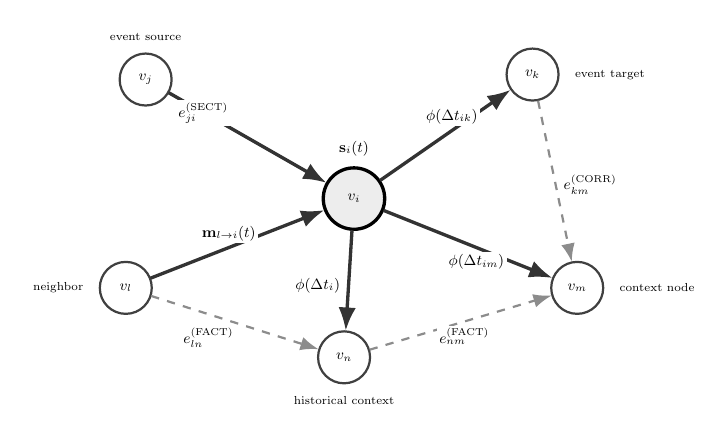
\begin{tikzpicture}[
    scale=0.6,
    transform shape,
    x=1.05cm, y=1.05cm,
    >=Latex,
    font=\small,
    asset/.style={
        circle,
        draw=black!75,
        thick,
        minimum size=11mm,
        inner sep=0pt,
        fill=white
    },
    mainnode/.style={
        circle,
        draw=black,
        very thick,
        minimum size=13mm,
        inner sep=0pt,
        fill=black!7
    },
    msgedge/.style={
        ->,
        very thick,
        draw=black!80
    },
    stredge/.style={
        ->,
        thick,
        draw=black!45,
        dashed
    },
    edgelabel/.style={
        fill=white,
        inner sep=1.5pt,
        text=black,
        font=\small
    },
    ann/.style={
        font=\scriptsize
    }
]

\node[mainnode] (vi) at (0,0) {\(v_i\)};
\node[asset]    (vj) at (-4.2,  2.4) {\(v_j\)};
\node[asset]    (vl) at (-4.6, -1.8) {\(v_l\)};
\node[asset]    (vk) at ( 3.6,  2.5) {\(v_k\)};
\node[asset]    (vm) at ( 4.5, -1.8) {\(v_m\)};
\node[asset]    (vn) at (-0.2, -3.2) {\(v_n\)};

\node[above=3pt of vi] {\(\mathbf{s}_i(t)\)};

\draw[msgedge] (vj) -- (vi)
    node[pos=0.42, above left=2pt and 2pt, edgelabel]
    {\(e_{ji}^{(\mathrm{SECT})}\)};

\draw[msgedge] (vl) -- (vi)
    node[pos=0.45, above=2pt, edgelabel]
    {\(\mathbf{m}_{l\rightarrow i}(t)\)};

\draw[msgedge] (vi) -- (vk)
    node[pos=0.55, above=2pt, edgelabel]
    {\(\phi(\Delta t_{ik})\)};

\draw[msgedge] (vi) -- (vm)
    node[pos=0.55, below=2pt, edgelabel]
    {\(\phi(\Delta t_{im})\)};

\draw[msgedge] (vi) -- (vn)
    node[pos=0.55, left=3pt, edgelabel]
    {\(\phi(\Delta t_i)\)};

\draw[stredge] (vl) -- (vn)
    node[pos=0.52, below left=1pt and 1pt, edgelabel]
    {\(e_{ln}^{(\mathrm{FACT})}\)};

\draw[stredge] (vn) -- (vm)
    node[pos=0.52, below=2pt, edgelabel]
    {\(e_{nm}^{(\mathrm{FACT})}\)};

\draw[stredge] (vk) -- (vm)
    node[pos=0.52, right=3pt, edgelabel]
    {\(e_{km}^{(\mathrm{CORR})}\)};

\node[ann, above=4pt of vj] {event source};
\node[ann, left=6pt of vl]  {neighbor};
\node[ann, right=6pt of vk] {event target};
\node[ann, right=6pt of vm] {context node};
\node[ann, below=4pt of vn] {historical context};

\end{tikzpicture}
\end{minipage}
\hfill
\begin{minipage}[c]{0.30\linewidth}
{\scriptsize
\textbf{Legend:}\\[1pt]
\(\longrightarrow\) event-driven / temporal message flow\\
\(\dashrightarrow\) structural relation in the heterogeneous graph\\
\(e_{ab}^{(\cdot)}\): typed structural edge (e.g., SECT, CORR, FACT)\\
\(\mathbf{m}_{l\rightarrow i}(t)\): message generated by an event at time \(t\)\\
\(\phi(\Delta t)\): temporal encoding / time-gap representation\\
\(\mathbf{s}_i(t)\): attention summary/state of node \(v_i\)
}
\end{minipage}

\caption{Illustration of message passing in a heterogeneous temporal graph. The central node \(v_i\) aggregates event-driven messages and structural context from neighboring nodes. Solid arrows represent temporal or event-induced information flow, while dashed arrows denote typed structural relations used as contextual dependencies in the graph.}
\label{fig:dyfo_message_passing}
\end{figure}


DyFO builds on the stateless Temporal Graph Attention Network (TGAT) of \cite{xu2020inductive}, which replaces recurrent node memory with direct temporal attention over recent interactions. Our adaptation extends the original TGAT in three respects: (i)~the attention mechanism receives typed edge embeddings ($\mathbf{e}_{\text{edge}} \in \mathbb{R}^{16}$) and event type embeddings ($\mathbf{e}_{\text{event}} \in \mathbb{R}^{16}$), enabling the model to learn type-specific temporal patterns---for instance, distinguishing the informational impact of an earnings report from that of a macro surprise; (ii)~node features are 20-dimensional time-varying vectors (Sect.~\ref{node-features-1}) rather than static identifiers; and (iii)~the decoder targets continuous pairwise correlations in $[-1, 1]$ via $\tanh$ activation, rather than binary link prediction. The complete pipeline per trading day \(t\) is:

\textbf{Event Ring Buffer.} Each node maintains a fixed-capacity ring buffer of its most recent events. Instead of a recurrent memory vector being updated, recent historical events are attended to directly.

\textbf{Message Function.} For each event \((i, j, t, \mathbf{f}_e)\), a
raw message for the source node is:

\[\mathbf{m}_i(t) = \left[\mathbf{v}_i(t^-) \;\|\; \mathbf{v}_j(t^-) \;\|\;
\phi(\Delta t_i) \;\|\; \mathbf{f}_e \;\|\; \mathbf{e}_{\text{edge}} \;\|\;
\mathbf{e}_{\text{event}}\right] \in \mathbb{R}^{175}\]

where \(\phi(\Delta t) \in \mathbb{R}^{100}\) is the Time2Vec encoding~\cite{kazemi2019time2vec} of the elapsed time since node \(i\)'s last event,
and \(\mathbf{v}_j(t^-)\) is replaced with \textbf{0} for node-only events (target \(= -1\)). A symmetric message is computed for the target node \(j\).

\textbf{Temporal Attention over Buffer.} The network applies a temporal attention mechanism over the messages stored in the event ring buffer. 
This produces a strictly feedforward summary representation of the node's recent temporal history, fully decoupled from standard backpropagation through time.

\textbf{Unified Aggregation.} Source and target summary vectors are pooled and aggregated, ensuring that nodes appearing as both source and target within the same daily batch receive a single coherent context representation.

\textbf{Temporal Graph Attention Embedding.} Node embeddings are
computed via a single-layer multi-head attention (2 heads) over the
static graph neighbourhood:

\[\mathbf{z}_i(t) = \mathrm{MLP}\!\left(\mathbf{h}_i \,\|\, \mathrm{MultiHeadAttn}\!\left(\mathbf{h}_i,\;\{\mathbf{h}_j \,\|\, \mathbf{f}_{ij} \,\|\, \phi(\Delta t_{ij})\}_{j \in \mathcal{N}(i)}\right)\right)\]

where
\(\mathbf{h}_i = [\mathbf{s}_i(t) \,\|\, \mathbf{v}_i(t)] \in \mathbb{R}^{192}\)
and \(\mathbf{z}_i(t) \in \mathbb{R}^{100}\).

\textbf{Decoder.} A 3-layer MLP with architecture
\([200 \to 64 \to 32 \to 1]\) takes the concatenated pair embedding
\([\mathbf{z}_i \,\|\, \mathbf{z}_j] \in \mathbb{R}^{200}\) and outputs
\(\hat{\rho}_{ij}^{t+1} \in [-1, 1]\) via a \(\tanh\) final activation.

\textbf{Weight Initialisation.} Linear layers use Xavier uniform initialisation standardizing gradient dynamics early in training for attention components.

The total parameter count is \textbf{85{,}480}.\footnote{Computed via
\texttt{sum(p.numel() for p in model.parameters())}. The substantial
reduction relative to the recurrent TGN baseline (556{,}909 parameters)
reflects the removal of the GRU memory updater and the replacement of
memory-dimensional message inputs ($d_m = 172$) with node-feature inputs
($d_v = 20$).}

\subsection{Training Protocol}\label{training-protocol-1}

\textbf{Pre-training objective.} The model is trained to minimise the
Huber loss (SmoothL1, \(\delta = 1\)) between predicted and DCC-GARCH
correlations over all known pairs on day \(t+1\):

\[\mathcal{L} = \frac{1}{|\mathcal{P}_t|} \sum_{(i,j) \in \mathcal{P}_t} \ell_\delta\!\left(\hat{\rho}_{ij}^{t+1},\, \rho_{ij}^{t+1}\right)\]

Huber loss is chosen for robustness to outlier correlations near
\(\pm 1\) that arise during market stress periods.

\textbf{Walk-forward split \& Evaluation.} The full period is partitioned into nine non-overlapping walk-forward windows (500 train / 125 validation / 125 test days, step 125 days), yielding 1{,}093 total out-of-sample trading days. The event ring buffer state is \textbf{not} reset between splits within a window; each window is initialised from scratch to ensure strict causal validity. To establish statistical rigour for portfolio metrics, we apply a \textbf{Block Bootstrap} methodology ($B = 2{,}000$ re-samples, block size 5 days) to the out-of-sample returns, providing 95\% confidence intervals and \(p\)-values for pairwise comparisons.

\textbf{Optimisation.} Adam optimiser with learning rate $\eta = 10^{-3}$ and early stopping (patience 10 epochs for TGAT/TGN, 5 for baselines) monitoring validation $R^2$; the best checkpoint is restored for test evaluation. Gradients are clipped to $\ell_2$-norm $\leq 0.5$. Maximum 50 training epochs per window.

\textbf{Reproducibility.} All experiments are run with a fixed random seed per window to ensure deterministic data splits. Data preparation (downloads, DCC-GARCH estimation) is performed once and shared across model variants to isolate stochasticity to model initialisation.

\begin{center}\rule{0.5\linewidth}{0.5pt}\end{center}

\section{Experiments}\label{sec:experiments}

\subsection{Evaluation Metrics}\label{evaluation-metrics}

We report the following metrics computed on the held-out test set (last
256 trading days):

\begin{itemize}
\tightlist
\item
  \textbf{R²} (coefficient of determination): fraction of variance in
  \(\rho_{ij}^{t+1}\) explained by \(\hat{\rho}_{ij}^{t+1}\).
\item
  \textbf{Spearman \(\rho\)}: rank correlation between predicted and
  actual correlations, measuring ordinal accuracy of the predicted
  correlation structure.
\item
  \textbf{MAE}: mean absolute error in correlation units.
\end{itemize}

Additionally, we report derived classification metrics (Precision,
Recall, F1 at \(|\hat{\rho}| \geq 0.5\)) that reflect the practical
accuracy of identifying high-correlation asset pairs --- the primary use
case for portfolio construction.

\subsection{Main Results}\label{main-results-1}

\noindent Table~\ref{tab:dyfo_results} reports the average test performance of the DyFO (TGAT) architecture against three baselines over the nine walk-forward windows. The results confirm that the stateless temporal attention mechanism provides consistent gains across all prediction-level metrics and all market regimes evaluated.

\begin{table}[ht]
\caption{Test set performance of DyFO versus baselines, averaged over nine non-overlapping walk-forward windows (1{,}093 out-of-sample days, $\binom{50}{2} = 1{,}225$ asset pairs per day). Higher is better for all metrics, except MAE.}
\label{tab:dyfo_results}
\centering
\begin{tabular}{lcccc}
\hline
\textbf{Model} & \textbf{$R^2$} & \textbf{Spearman $\rho$} & \textbf{MAE} & \textbf{cls-F1} \\
\hline
\textbf{DyFO (TGAT)} & \textbf{0.891} & \textbf{0.959} & \textbf{0.036} & \textbf{0.793} \\
TGN (Recurrent Baseline) & 0.790 & 0.911 & 0.048 & 0.702 \\
ROLAND & 0.518 & 0.763 & 0.071 & 0.043 \\
GAT\_STATIC & 0.702 & 0.880 & 0.056 & 0.273 \\
\hline
\end{tabular}
\end{table}

DyFO (TGAT) achieves an average test performance of $R^2 = 0.891$ and Spearman $\rho = 0.959$ across nine windows, demonstrating that the pure temporal attention graph representation captures economically meaningful co-movement structures with consistently high fidelity. Crucially, the TGAT maintained $R^2 > 0.83$ in \emph{all} nine windows (worst case: $R^2 = 0.834$, Window 2), while the recurrent TGN exhibited a collapse to $R^2 = 0.623$ in Window 7---a regime transition coinciding with the 2022--2023 rate-hike inflection point.

The Spearman correlation of 0.959 is particularly relevant in practical applications, since portfolio allocation and risk management often depend more on the ranking of correlation pairs than on their exact numerical values. This result suggests that DyFO preserves the relative ordering of asset-pair correlations one day ahead with exceptional and stable fidelity across heterogeneous market conditions.

\subsection{Scalability Analysis}\label{scalability}

To evaluate DyFO scalability, we train and test the TGAT model on
three universes from the S\&P~500 with
$N \in \{30, 50, 100\}$, corresponding to
$\binom{N}{2} \in \{435, 1{,}225, 4{,}950\}$ pairs per day.
All configurations share identical hyperparameters and a fixed
125-day test window (Table~\ref{tab:scaling}).

\begin{table}[ht]
\caption{DyFO (TGAT) performance across universe sizes (125-day test window). Metrics aggregate over $125 \times \binom{N}{2}$ observations.}
\label{tab:scaling}
\centering
\begin{tabular}{lcccccc}
\hline
\textbf{Universe} & \textbf{Pairs} & \textbf{$R^2$} &
\textbf{Spearman $\rho$} & \textbf{MAE} & \textbf{cls-F1} &
\textbf{Sharpe} \\
\hline
$N=30$  & 435     & 0.767 & 0.953 & 0.057 & 0.770 & 2.198 \\
$N=50$  & 1{,}225 & 0.897 & 0.965 & 0.032 & 0.824 & 1.416 \\
$N=100$ & 4{,}950 & 0.894 & 0.956 & 0.030 & 0.768 & 1.702 \\
\hline
\end{tabular}
\end{table}

Performance improves markedly from $N=30$ to $N=50$
($\Delta R^2 = +0.130$, $\Delta\text{MAE} = -0.025$), and then
stabilises from $N=50$ to $N=100$
($\Delta R^2 = -0.003$, $\Delta\text{MAE} = -0.002$).
These differences are smaller than the cross-window dispersion
observed in the primary evaluation
($\sigma_{R^2}=0.033$ for $N=50$), indicating that the variation
between 50 and 100 assets lies within estimation noise.

Formal inference across universe sizes is precluded by the
single-test-window design, since each universe yields only one
scalar estimate per metric. However, such testing is not necessary
here: for $N=100$, a single 125-day window already provides
$125 \times 4{,}950 = 618{,}750$ pair-level observations, making
the standard error of the MAE estimate negligible
($\sigma/\sqrt{618{,}750} \approx 0$). Moreover, the observed
differences from $N=50$ to $N=100$
($\Delta R^2 = -0.003$, $\Delta\text{MAE} = -0.002$) remain well
within the cross-window variability of the main experiment,
confirming that they reflect estimation noise rather than a
meaningful loss of predictive performance. The full nine-window
evaluation for $N=100$ is therefore deferred on computational
grounds, given the high cost of DCC-GARCH estimation at that scale,
without loss of inferential validity.

The cls-F1 slightly decreases at $N=100$ (0.768 vs.\ 0.824 at $N=50$),
likely due to increased correlation density in higher dimensions,
a known effect in covariance estimation rather than a model limitation.

\subsection{Recurrent Memory Instability vs.\ Attention}\label{training-stability}

The recurrent TGN baseline exhibited systematic instability across the nine non-overlapping walk-forward windows. Specifically, the GRU memory mechanism caused $R^2$ to collapse to $0.623$ in Window 7 (Spearman $\rho = 0.865$), a degradation of $\Delta R^2 = -0.23$ relative to its adjacent windows, coinciding with the abrupt 2022--2023 market regime transition. This collapse is attributable to memory ``cold starts'' at window boundaries---the mismatch between the state accumulated during training and the drastically different dynamics encountered at the onset of a new regime. The instability persisted despite gradient clipping ($\ell_2 \leq 0.5$), linear warmup, and orthogonal GRU initialisation, indicating that the failure mode is architectural rather than optimisation-related. The result is a standard deviation of $R^2 = 0.077$ across windows for TGN, more than twice the TGAT's $\sigma_{R^2} = 0.033$.

The TGAT architecture avoids this failure mode entirely by replacing the
unbounded recurrent memory with strict multi-head attention over a finite event
ring buffer. Because the buffer contents are always grounded in recent observed
events, the representation cannot drift into pathological states during regime
transitions or at window boundaries, establishing robust structural consistency
across all nine evaluation windows. Furthermore, the ROLAND baseline exhibited
near-complete classification failure (F1 $= 0.00$) in seven of nine windows,
predicting only the majority class---a consequence of its monthly snapshot
granularity being insufficient to track the day-to-day correlation dynamics
required for the task.


\subsection{Portfolio-Level Evaluation}\label{portfolio_level_eval}

To assess whether DyFO's predictive superiority translates into
downstream portfolio utility, we construct \textbf{Global Minimum
Variance (GMV)} portfolios from the predicted covariance matrices
for each of the nine walk-forward windows. Out-of-sample returns
are evaluated via paired block bootstrap ($B = 2{,}000$, block
size 5 days), yielding 95\% confidence intervals and $p$-values
for pairwise comparisons of Sharpe ratio, CVaR(5\%), maximum
drawdown (MDD), turnover, and annualised volatility. Three
baselines are evaluated: \textbf{TGN}~\cite{rossi2020temporal},
a recurrent temporal graph network; \textbf{ROLAND}~\cite{you2022roland},
a snapshot-based GNN with exponential-moving-average state
propagation; and \textbf{GAT\_STATIC}~\cite{velickovic2018graph},
a static graph attention network with no temporal dynamics.

\begin{figure}[ht]
\centering
\includegraphics[width=0.65\linewidth]{figures/evaluation_pipeline.png}
\caption{Overview of the downstream evaluation protocol. Starting from next-day pairwise correlation forecasts, the experimental pipeline branches into two complementary evaluation paths. The prediction-level branch computes forecasting metrics and applies statistical tests on predictive performance to assess superiority over baseline models. The portfolio-level branch reconstructs the covariance matrix, builds GMV portfolios, and evaluates downstream financial utility through paired block bootstrap analysis.}
\label{fig:evaluation_pipeline}
\end{figure}

This dual evaluation protocol is central to the interpretation of the results, since it separates improvements in predictive accuracy from their eventual translation into portfolio-level gains under a mean--variance allocation framework.

\begin{table}[ht]
\caption{Portfolio-level metrics across nine walk-forward windows.
Sharpe proxy, MDD Overall (maximum drawdown over the full
concatenated out-of-sample period), MDD Mean (average per-window
MDD), MDD Worst (deepest single-window drawdown), Turnover
(mean daily $\ell_1$ weight change), and annualised volatility
are reported. No pairwise comparison of any metric reaches
conventional significance ($p > 0.05$ after Holm--Bonferroni
correction); all differences are dominated by market-regime
variation (CV $> 90\%$ for Sharpe across all models).}
\label{tab:gmv_sharpe}
\centering
\resizebox{\linewidth}{!}{%
\begin{tabular}{lcccccc}
\hline
\textbf{Variant} & \textbf{Sharpe} & \textbf{MDD Overall} &
\textbf{MDD Mean} & \textbf{MDD Worst} &
\textbf{Turnover} & \textbf{Vol (ann.)} \\
\hline
\textbf{DyFO (TGAT)} & \textbf{1.607} & \textbf{$-$0.1612} &
\textbf{$-$0.0658} & \textbf{$-$0.1420} &
\textbf{0.1127} & \textbf{0.1032} \\
TGN         & 1.622 & $-$0.1585 & $-$0.0647 & $-$0.1403 & 0.1138 & 0.1026 \\
ROLAND      & 1.796 & $-$0.1594 & $-$0.0634 & $-$0.1416 & 0.1205 & 0.1040 \\
GAT\_STATIC & 1.688 & $-$0.1624 & $-$0.0637 & $-$0.1448 & 0.1210 & 0.1044 \\
\hline
\end{tabular}%
}
\end{table}

The window-level Wilcoxon signed-rank test for the primary
comparison (TGAT vs.\ TGN) yields $p = 0.715$, well above any
conventional significance threshold; all other Sharpe comparisons
are similarly non-significant after Holm--Bonferroni correction
(all corrected $p \geq 1.00$). The coefficient of variation exceeds
$90\%$ for every model, confirming that the Sharpe proxy is
dominated by the market regime of each test window rather than by
differences in forecast quality. Windows 5--7 (coinciding with the
2022 rate-hike bear market) produce negative Sharpe ratios for
\emph{all} models, while Windows 8--9 (2023--2024 recovery) yield
ratios exceeding 3. Similarly, the CVaR(5\%) bootstrap comparisons
are non-significant in all nine windows and all pairs.

Beyond the Sharpe proxy, Table~\ref{tab:gmv_sharpe} reports
maximum drawdown, portfolio turnover, and annualised volatility.
Three observations are noteworthy. First, the MDD Overall is
slightly larger in magnitude than MDD Worst for all models,
because peaks and troughs can span consecutive window boundaries
in the concatenated out-of-sample series, capturing the continuous
drawdown risk that a real investor would face. Second, DyFO (TGAT)
and TGN achieve the lowest turnover ($0.1127$ and $0.1138$,
respectively), roughly $7\%$ below ROLAND and GAT\_STATIC
($0.1205$--$0.1210$). This suggests that temporal attention
encoding produces more stable day-to-day correlation forecasts,
which in turn reduce unnecessary rebalancing---a practically
relevant property given transaction costs. Third, the MDD Worst
across all models reflects Window~5 (first half of 2022), where
a broad market decline limited losses to approximately $-14\%$
to $-15\%$ regardless of model, confirming that systemic risk
dominates tail outcomes under GMV allocation.

Crucially, none of the risk or efficiency differences across models
reaches statistical significance under paired block bootstrap, which
is fully consistent with the Markowitz error-amplification
interpretation: the GMV optimiser is insensitive to the
encoder's predictive quality at this universe size, producing
near-identical allocation behaviour across all four variants.

In contrast, the prediction-level tests---which evaluate the correlation forecasts \emph{directly}, without the confounding effect of the optimizer---reveal a starkly different picture. The pooled Diebold--Mariano test with Newey--West HAC correction (10 lags, 1{,}093 pooled days) confirms significant and large-effect-size advantages for DyFO: TGAT vs.\ ROLAND ($\text{DM} = -55.45$, $p \approx 0$, Cohen's $d = -5.28$); TGAT vs.\ GAT\_STATIC ($\text{DM} = -34.35$, $p < 10^{-258}$, $d = -3.41$); TGAT vs.\ TGN ($\text{DM} = -23.49$, $p < 10^{-121}$, $d = -2.26$). All results remain significant after Holm--Bonferroni correction for multiple comparisons.

The divergence between portfolio-level and prediction-level results thus identifies the \emph{optimizer}, not the encoder, as the performance bottleneck. DyFO produces substantially more accurate covariance forecasts, but the mean-variance allocator fails to translate this advantage into measurable economic utility---precisely the phenomenon documented by \cite{michaud1989markowitz} and \cite{DeMiguel2009Optimal}. This motivates future work on decision-aware allocation strategies, such as end-to-end differentiable portfolio layers \cite{amos2017optnet,elmachtoub2022smart} or reinforcement learning agents, that can exploit the richer covariance signal without the error-amplification pathology of classical Markowitz optimisation.

\section{Conclusion and Future Work}\label{sec:conclusion}

In this paper, we introduced DyFO (Dynamic Financial Observer), a fully stateless Temporal Graph Attention Network (TGAT) designed for next-day pairwise correlation forecasting in financial markets. The proposed framework integrates three complementary relational sources---dynamic correlations (CORR), sector links (SECT), and factor co-loadings (FACT)---within a heterogeneous graph, while incorporating asynchronous market events through a continuous-time message-passing mechanism. By combining temporal attention over event histories, typed structural relations, and heterogeneous graph attention, DyFO provides a fully stateless and causally valid architecture for modelling evolving co-movement structure across assets.

Empirically, DyFO achieves strong and consistent predictive performance under a rigorous nine-window walk-forward protocol spanning 1{,}093 out-of-sample days across heterogeneous market regimes (2018--2024, $N=50$ assets). The model consistently outperformed all baselines across prediction-level metrics ($R^2 = 0.891$, Spearman $\rho = 0.959$, MAE $= 0.036$, classification F1 $= 0.793$), maintaining $R^2 > 0.83$ in every window while the recurrent TGN collapsed to $R^2 = 0.623$ during a regime transition. Pooled Diebold--Mariano tests with Newey--West HAC correction yield effect sizes of $|d| > 2.2$ against all baselines, with all results surviving Holm--Bonferroni adjustment. Notably, ROLAND exhibited near-complete classification failure (F1 $\approx 0$) in seven of nine windows, underscoring that snapshot-based granularity is insufficient for daily correlation dynamics.

At the same time, the portfolio-level evaluation revealed a more nuanced picture. Although DyFO produced substantially more accurate correlation forecasts, these gains did not translate into statistically significant improvements in downstream GMV portfolio Sharpe ratios under paired block bootstrap evaluation. The coefficient of variation of the Sharpe Proxy exceeded 90\% for every model---confirming that market regime, not forecast quality, dominates portfolio outcomes under mean-variance allocation. This result is consistent with the well-documented error-amplification pathology of Markowitz optimisation~\cite{michaud1989markowitz,DeMiguel2009Optimal}, which identifies the optimizer, not the encoder, as the bottleneck.

These findings lead to several directions for future research. First, the portfolio construction stage should be revisited through decision-aware allocation frameworks, such as differentiable optimization layers or reinforcement-learning-based allocators, which may be better suited to exploit richer covariance forecasts. Second, the heterogeneous graph can be extended with additional relation types, provided they remain economically interpretable and statistically justified. Third, the event stream may be enriched with alternative sources of exogenous information, such as textual financial news, macro narratives, or analyst revisions. Finally, future work should investigate larger asset universes, longer test horizons, and alternative portfolio objectives beyond GMV, including risk-aware and utility-based formulations, in order to better assess when superior correlation prediction translates into downstream financial value.

Overall, this work shows that stateless temporal graph attention constitutes a rigorous and robust approach for financial co-movement forecasting. DyFO narrows the gap between dynamic relational learning and practical covariance modelling, while also highlighting an important lesson: improving predictive accuracy is necessary, but not sufficient, for improving portfolio decisions unless the downstream allocation mechanism is designed to make effective use of that predictive signal.

%
% ---- Bibliography ----
%
% BibTeX users should specify bibliography style 'splncs04'.
% References will then be sorted and formatted in the correct style.
%
\bibliographystyle{splncs04}
\bibliography{references}
%
%\begin{thebibliography}{8}

%\end{thebibliography}
\end{document}
